\documentclass[
	11pt,								% 11 Punkt Schrift verwenden (auch 10pt, 12pt moeglich)
	a4paper,						% Dokumentgroesse A4
	oneside,						% einseitiger Druck (auch twoside moeglich)
	titlepage,					% Titelblatt generieren
	headsepline,				% Kopfzeile duch Linie vom text getrennt
	DIV13,							% Groesse des Satzspiegels
	abstracton,	 				% zeigt die Abstractueberschrift (abstracton oder abtractoff)
	BCOR0cm,						% Groesse des Bindungsrandes (z. B.: BCOR2.5cm)
	bibliography=totoc, % bibliography is added to the table of contents
]{scrreprt}							% Dokumentenklasse (KomaScript - Report)
%]{report}							% Dokumentenklasse (Native Latex - Report)

% MATH, FORMULAE AND SIGNS PACKAGES
\usepackage{amsmath}								% besser als standard math
\usepackage{amssymb}

% LANGUAGE PACKAGES
%\usepackage[german]{				% Anpassungen ensprechend der Sprache
%\usepackage[latin1]{inputenc}
\usepackage[ngerman]{babel}
\usepackage[T1]{fontenc}

\usepackage[utf8]{inputenc}				% direkte Eingabe von Umlauten
\usepackage{csquotes}							% Anfuehrungszeichen entsprechend der Sprache

% GRAPHIC PACKAGES
\usepackage{graphicx}							 % Packet zu Einbindung von Graphiken
\usepackage{subfig}									% fuer die Erstellung von Unterabbildungen
\usepackage{wrapfig}

% LAYOUT PACKAGES
\usepackage{fancyhdr}
\usepackage{parskip}								% besseres Absatzlayout (Leerzeile statt Einrückung)
\usepackage[official,right]{eurosym}% für ein \euro{} Symbol
\usepackage{hyperref}							% F\"ur Hyperlinks
\hypersetup{
	hypertexnames=true,
	unicode = {true},
	colorlinks = {true},
	pdftitle = {Entwicklung eines Systems ...},
	pdfauthor = {Christian Schaub},
	pdfkeywords = {keywords},
	pdfborder = {0 0 0},
	linkcolor = black,
	citecolor = black,
	urlcolor = black,
	breaklinks = true,
}
\usepackage{url}										% fuer URLs als Literaturverzeichnis
\usepackage{color}
\usepackage{setspace}
\usepackage{rotfloat}
%\usepackage{verbatim}								% multiline comments
\usepackage{nextpage}
\usepackage[textsize=scriptsize]{todonotes}
\usepackage[numbers]{natbib}


%\usepackage[
%	block=nbpar,
%	citestyle=numeric-comp,
%	bibstyle=stopfer,
%	maxbibnames=10
%]{biblatex}
%\addbibresource{bibtex_database.bib}

% OPTIONS, DEFINITIONS
\usetikzlibrary{arrows,automata,shapes.multipart,trees}
\onehalfspacing							% anderthalbzeilig (oder auch \doublespace)
\pagestyle{headings}				% Überschrift in der Kopfzeile und Seitenzahlen
\setcapindent{0mm}
\addtokomafont{caption}{\small}

% OWN COMMANDS

% Adding lines above and below the chapter head
\newcommand*{\ORIGchapterheadstartvskip}{}
\let\ORIGchapterheadstartvskip=\chapterheadstartvskip
\renewcommand*{\chapterheadstartvskip}{
	 \ORIGchapterheadstartvskip{
			 \setlength{\parskip}{-40pt}
			 \noindent\rule{.3\textwidth}{3pt}\rule[2.5pt]{.7\linewidth}{.5pt}\par
	 }
}

\newcommand*{\ORIGchapterheadendvskip}{}
\let\ORIGchapterheadendvskip=\chapterheadendvskip
\renewcommand*{\chapterheadendvskip}{
	 {
			 \setlength{\parskip}{0pt}
			 \noindent\rule{.3\textwidth}{.5pt}\par
	 }
	 \ORIGchapterheadendvskip
}

\newcommand{\eclipse}{$\mbox{ECL}^i\mbox{PS}^e$}

%%%%%%%%%%%%%%%%%%%%%%%%%%%%%%%%%%%DOCUMENT%%%%%%%%%%%%%%%%%%%%%%%%%%%%%%%%%%%%%

\begin{document}

% Cover
	%\pagenumbering{alpha}
	\thispagestyle{empty}
	
\includegraphics[height=1.2cm]{images/vsLogo.png}
	\hfill
\includegraphics[height=1.2cm]{images/uniLogo.pdf}\\[1cm]

	\begin{center}
		\begin{LARGE}\bfseries Verteiltes Monitoring\end{LARGE}\\
		[2cm]
		\Large{Universität Kassel}\\
		[1cm]
		\large{Projektbericht von}\\
		\Large{Christian Schaub}\\
		[1cm]
		\large \Large{Fachgebiet Verteilte Systeme \\
		Universität Kassel}\\
		[1cm]
	\end{center}
	
%	\begin{abstract}
%	Kurze Beschreibung des Projektes
%	\end{abstract}


	\vfill
	\begin{Large}
		\begin{tabular}{l l}
			Gutachter: & Prof. Dr. Kurt Geihs\\
			[1cm]
			Betreuer: & Dipl.-Ing. Dominik Kirchner\\
		\end{tabular}
	\end{Large}
	\vfill

	\begin{center}Datum: Januar 21, 2013\end{center}

	

	\tableofcontents

	
	%% Hier können die einzelnen Kapitel inkludiert werden. Sie müssen in den 
% entsprechenden .TEX-Dateien vorliegen. Die Dateinamen können natürlich 
% angepasst werden.
%\include{Inhalt/Akronyme} %Akronyme.tex
\chapter{Related Work}
\label{cha:Related Work}

\section{Section 2}
\label{sec:2Section2}
Willkommen im Portal f"ur Elektronik, Maschinenbau und Mechatronik !
Dieses Portal soll euch beim lernen und diskutieren der einzelnen Studienf"acher behilflich sein, oder im Alltag als Knowledge-Base zur Verf"ugung stehen ! \\
F"ur jedes Studienfach wird in einem "Ubersichtsartikel der Inhalt zusammengefasst und die einzelnen Fachartikel in Beziehung zueinader gestellt. 
Kommen Formeln in den Fachartikeln vor, werden diese in einer Formelsammlung zu dem jeweiligen Studienfach zusammengef"uhrt. 
Am Ende soll jedes Studienfach eine"Ubersichtsartikel und wenn m"oglich eine Formelsammlung besitzen.

\subsection{Subcestion 2.1}
\label{subsec:2Subcestion2.1}

\begin{figure}[htb]
\centering
\includegraphics[width=0.2\textwidth]{mkDoc-Logo.png}
\caption{mkDoc}
\label{fig:mkDoc}
\end{figure}


\subsection{Subcestion 2.2}
\label{subsec:2Subcestion 2.2}
Willkommen im Portal f"ur Elektronik, Maschinenbau und Mechatronik !\footnote{\Vgl\Zitat[S.~11]{Sicherheitstechnik}}
Dieses Portal soll euch beim lernen und diskutieren der einzelnen Studienf"acher behilflich sein, oder im Alltag als Knowledge-Base zur Verf"ugung stehen ! \\
F"ur jedes Studienfach wird in einem "Ubersichtsartikel der Inhalt zusammengefasst und die einzelnen Fachartikel in Beziehung zueinader gestellt. 
Kommen Formeln in den Fachartikeln vor, werden diese in einer Formelsammlung zu dem jeweiligen Studienfach zusammengef"uhrt. 
Am Ende soll jedes Studienfach einen  "Ubersichtsartikel und wenn m"oglich eine Formelsammlung besitzen.

 %Einleitung.tex
\include{Inhalt/Relatedwork} %Vorgaben.tex
\include{Inhalt/Konzept} %Entwicklung.tex
\include{Inhalt/Umsetzung} %Umsetzung.tex
\include{Inhalt/Evaluierung} %Fazit.tex
\include{Inhalt/Zusammenfassung} %Zusammenfassung.tex

 %Inhalt.tex
\chapter{Einleitung}
\label{cha:Einleitung}

Im Fachgebiet Verteilte Systeme werden seit mehreren Jahren Möglichkeiten untersucht, autonome und teamfähige
Roboter zu entwickeln. Diese Roboterteams treten beispielsweise gegen Roboterteams anderer Universitäten im sogenannten RoboCup an. Der RoboCup ist eine Forschungsinitiative, die die Forschung im
Bereich autonomer Robotik fördert. Die autonomen Roboterteams treten hier gegeneinander in Fussballspielen an.\\

%Mit Forchungsgebiet autonome Roboter beginnen ... relevant ... viel untersucht ... vielleicht ein paar Referenzen dazu ... Dann dazu übergehen, dass gerade AUTONOMES verhalten sicherheitskritisch ist und überwacht werden muss ... 

Autonome Roboter erfordern eine verlässliche Sensorik und Aktorik um die Roboter selbst, sowie deren Nutzer oder auch Zuschauer während Vorführungen zu
schützen. Als Beispiel können die Fussballroboter des Fachgebietes, mit ca. 30kg Gewicht und einer maximalen Geschwindigkeit
von 4m/s (richtig ??) oder weitere autonome Roboter beispielsweise aus dem Rescue-Bereich dienen. Diese können durch ihren Aufbau, das damit
verbundene Gewicht und ihrer maximalen Geschwindigkeit auch eine Gefahr darstellen. Sämtliche Aktorik und Sensorik ist auf bestimmte physikalische Gegebenheiten angewiesen, um 
nach Spezifikation zu funktionieren. Viele Mikrocontroller, wie auch der in diesem Projekt eingesetzte ATMega644 benötigen beispielsweise eine stabilisierte Betriebsspannung von 3.3V oder 5V.\\
Im Rahmen dieses Projektes wurden daher Möglichkeiten untersucht physikalische Größen
in einem autonomen Robotersystem zu messen und direkt auf der Controllerebene entsprechende Reaktionen auszuführen. Die Reaktivität des Systems beschleunigt die Reaktion auf Messwerte, da die 
Datenverarbeitung nicht vom Robotersystem selbst, § weglassen ? z.B. ein Laptop oder Barebone mit Ubuntu System §, sondern direkt auf Controllerebene durchgeführt wird.
%passt so nicht ... gedanke sollte rein ... Würde anfangen mit ... verbindung zu vorherigen satz suchen: Schnelle Reaktion wichtig -> daher hohe reaktivität wichtig für projekt. Rest is für Einleitung zu viel detail
 Ein Beispiel wäre hier die sofortige Deaktivierung eines Sensors, sollte eine Betriebsspannung außerhalb der Spezifikation anliegen.
Dadurch könnten, durch die nicht korrekte Betriebsspannung verursachte fehlerhafte Messungen verhindert werden, noch bevor diese Daten das Robotersystem
erreichen. 
%hier betonen, dass die messdaten primär als "update der roboterinternen wissensbasis" (nicht so schreiben) benötigt werden und daher eine Kommunikation mit dem Steuer PC ein erforderliche Teilaufgabe des Projektes ist.

%Deinen Satz streichen
Des weiteren werden die Messwerte zur weiteren Verarbeitung redundant zum Robotersystem übermittelt. Zur Messung der Werte, Reaktion und
Kommunikation wurde eine zweischichtige Platine mit Steuer- und messteil sowie Software entwickelt. Auf die einzelnen Schritte vom Formulieren
der Problemstellung über konzeptionelle Entscheidungen bis zur Umsetzung und Evaluierung wird in den folgenden Kapiteln eingegangen.\\






Related Work:
-


% ab Einleitung zählen !!
\pagenumbering{arabic}




\chapter{Problemstellung}
\label{cha:Problemstellung}
Autonome Roboter bestehen aus mechanischen und elektronischen Komponenten und sind, wie einleitend beschrieben, 
schnell und schwer genug um sich selbst, Nutzer oder sonstige Gegenstände in der Umgebung zu schädigen. 
Ziel dieses Projektes ist eine Verbesserung der Verläßlichkeit eines autonomen Roboters, indem es ermöglicht wird 
physikalische Größen\footnote{elektronische Spannung, Temperatur} zu messen, deren Auswirkungen wichtige mechanische oder elektronische Komponenten beeinflussen können. 
Anschliessed sollen mittels der erfassten Daten Schlussfolgerungen über den Zustand der überwachten Komponenten gezogen und dementsprechend im Fehlerfall
 direkte Reaktionen des Meßsystems durchgeführt werden können. 
§  Durch eine derartige Reaktion muß beispielsweise der Hardreset\footnote{kurzzeitige Unterbrechung der Spannungsversorgung} oder 
die Deaktivierung eines anderen Controllers durchgeführt werden können. § 
Des weiteren muß eine Verbindung zur Kommunikation zwischen dem Roboter- und Meßsystem ermöglicht werden, um einerseits die 
erfassten Daten dem Robotersystem übermitteln zu können und andererseits die Einstellung bestimmter Parameter, sowie die Steuerung der Aktionen des Meßsystems durch das Robotersystem ermöglichen.

\begin{figure}[htb]
\centering
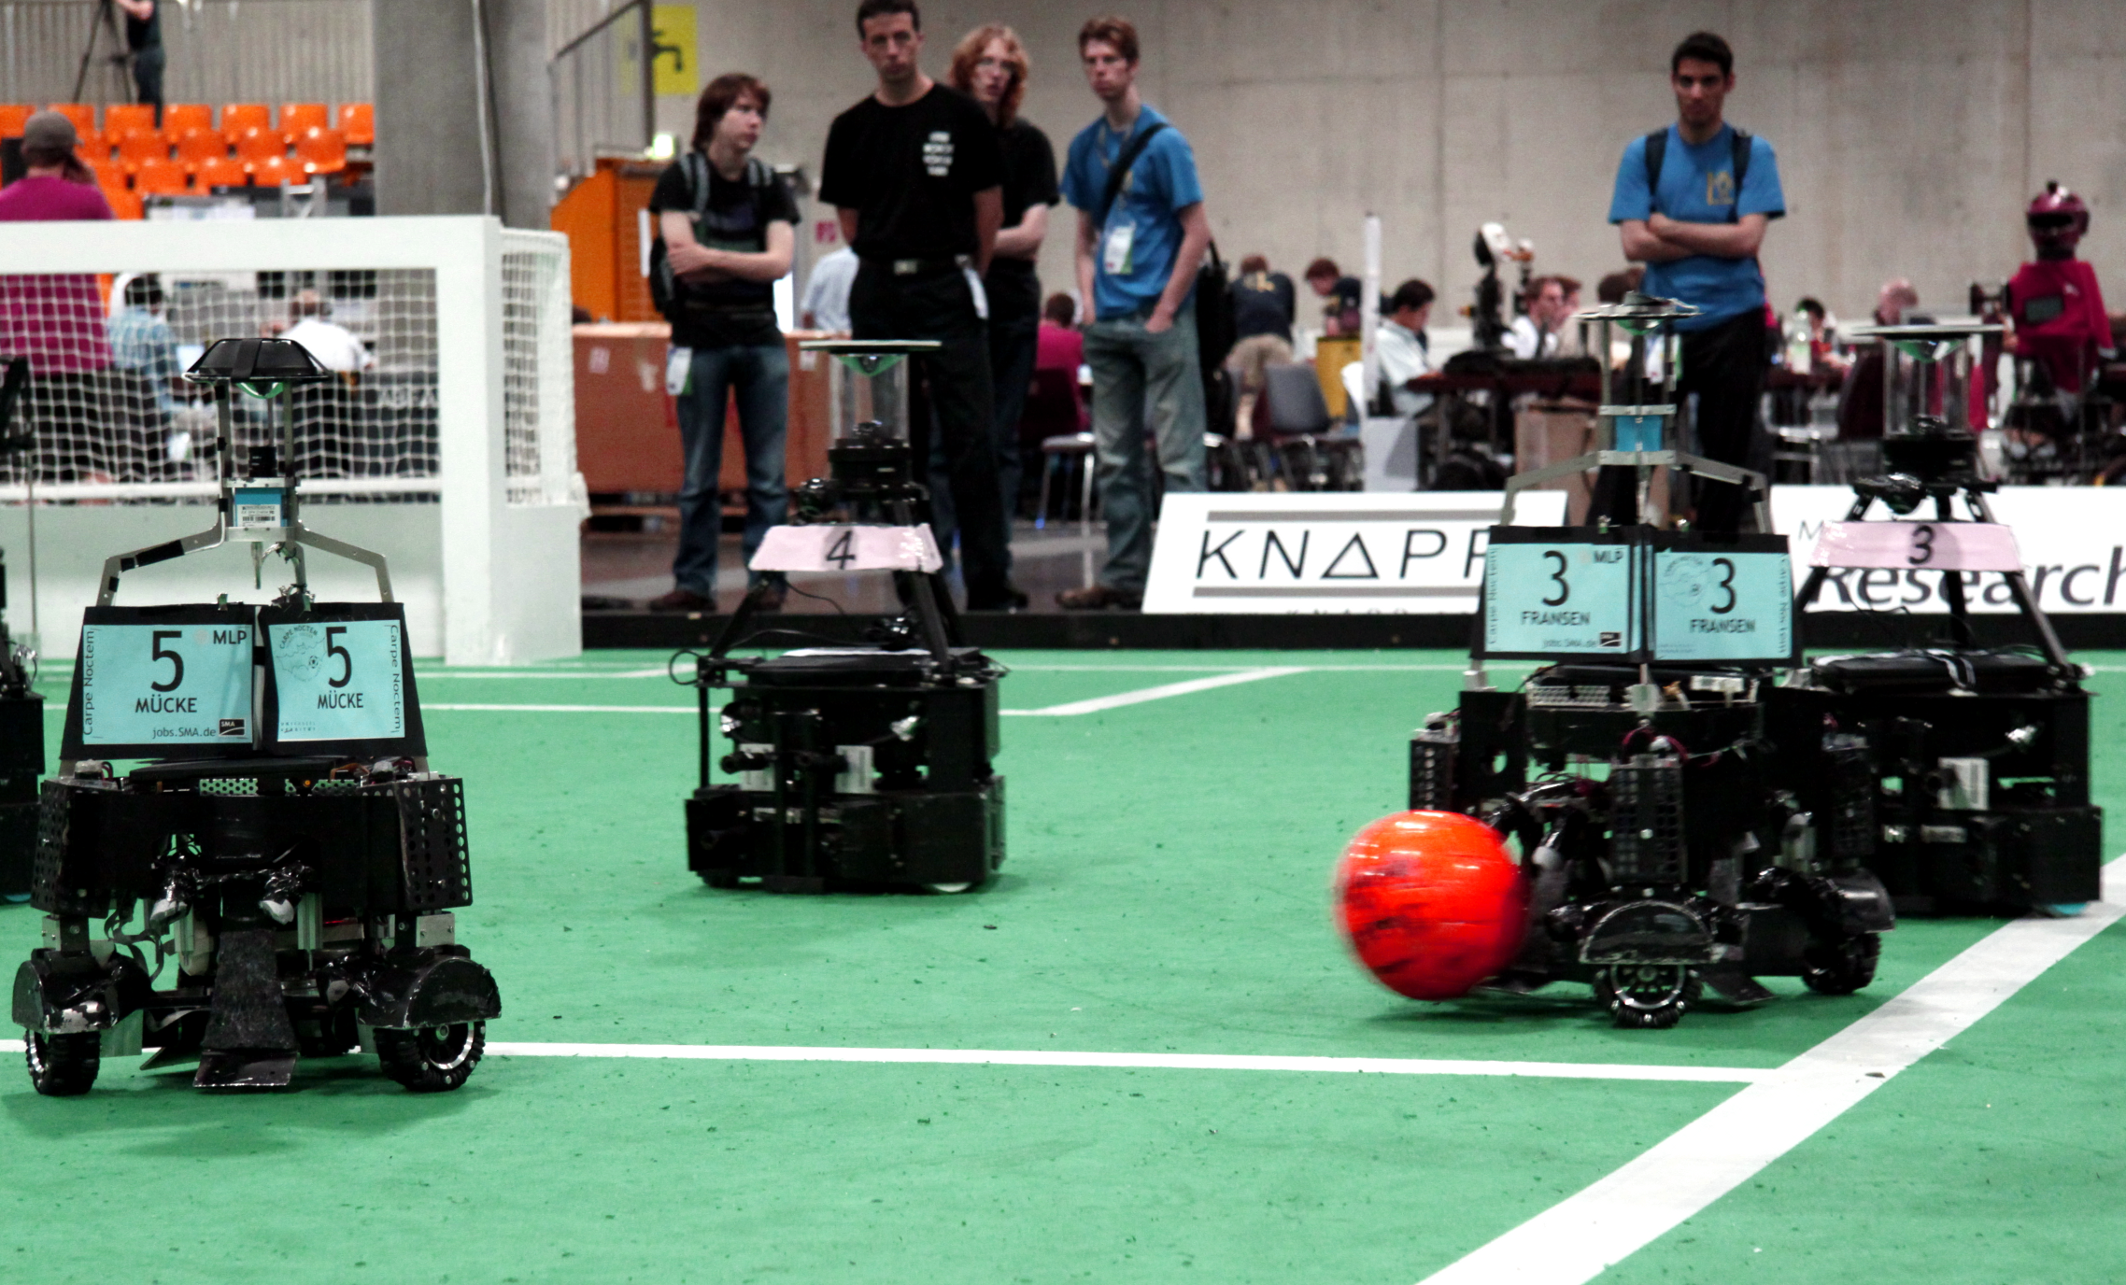
\includegraphics[width=0.8\textwidth]{images/robots.png}
\caption{Roboter Unfall}
\label{fig:Roboter Unfall}
\end{figure}

% \begin{wrapfigure}{r}{0 cm}
%%%%%%%%%%%%%%%%%%%%%%%%%%%%%%%%%%%%%%%%%%%%%%%%%%%%%%%%%%%%%%%%%%%%%%%%%%%%%%%%%%%%%%%
%%% You will need to add \usepackage{wrapfig} to your preamble to use textwrapping %%%
%%%%%%%%%%%%%%%%%%%%%%%%%%%%%%%%%%%%%%%%%%%%%%%%%%%%%%%%%%%%%%%%%%%%%%%%%%%%%%%%%%%%%%%
% \centering
 %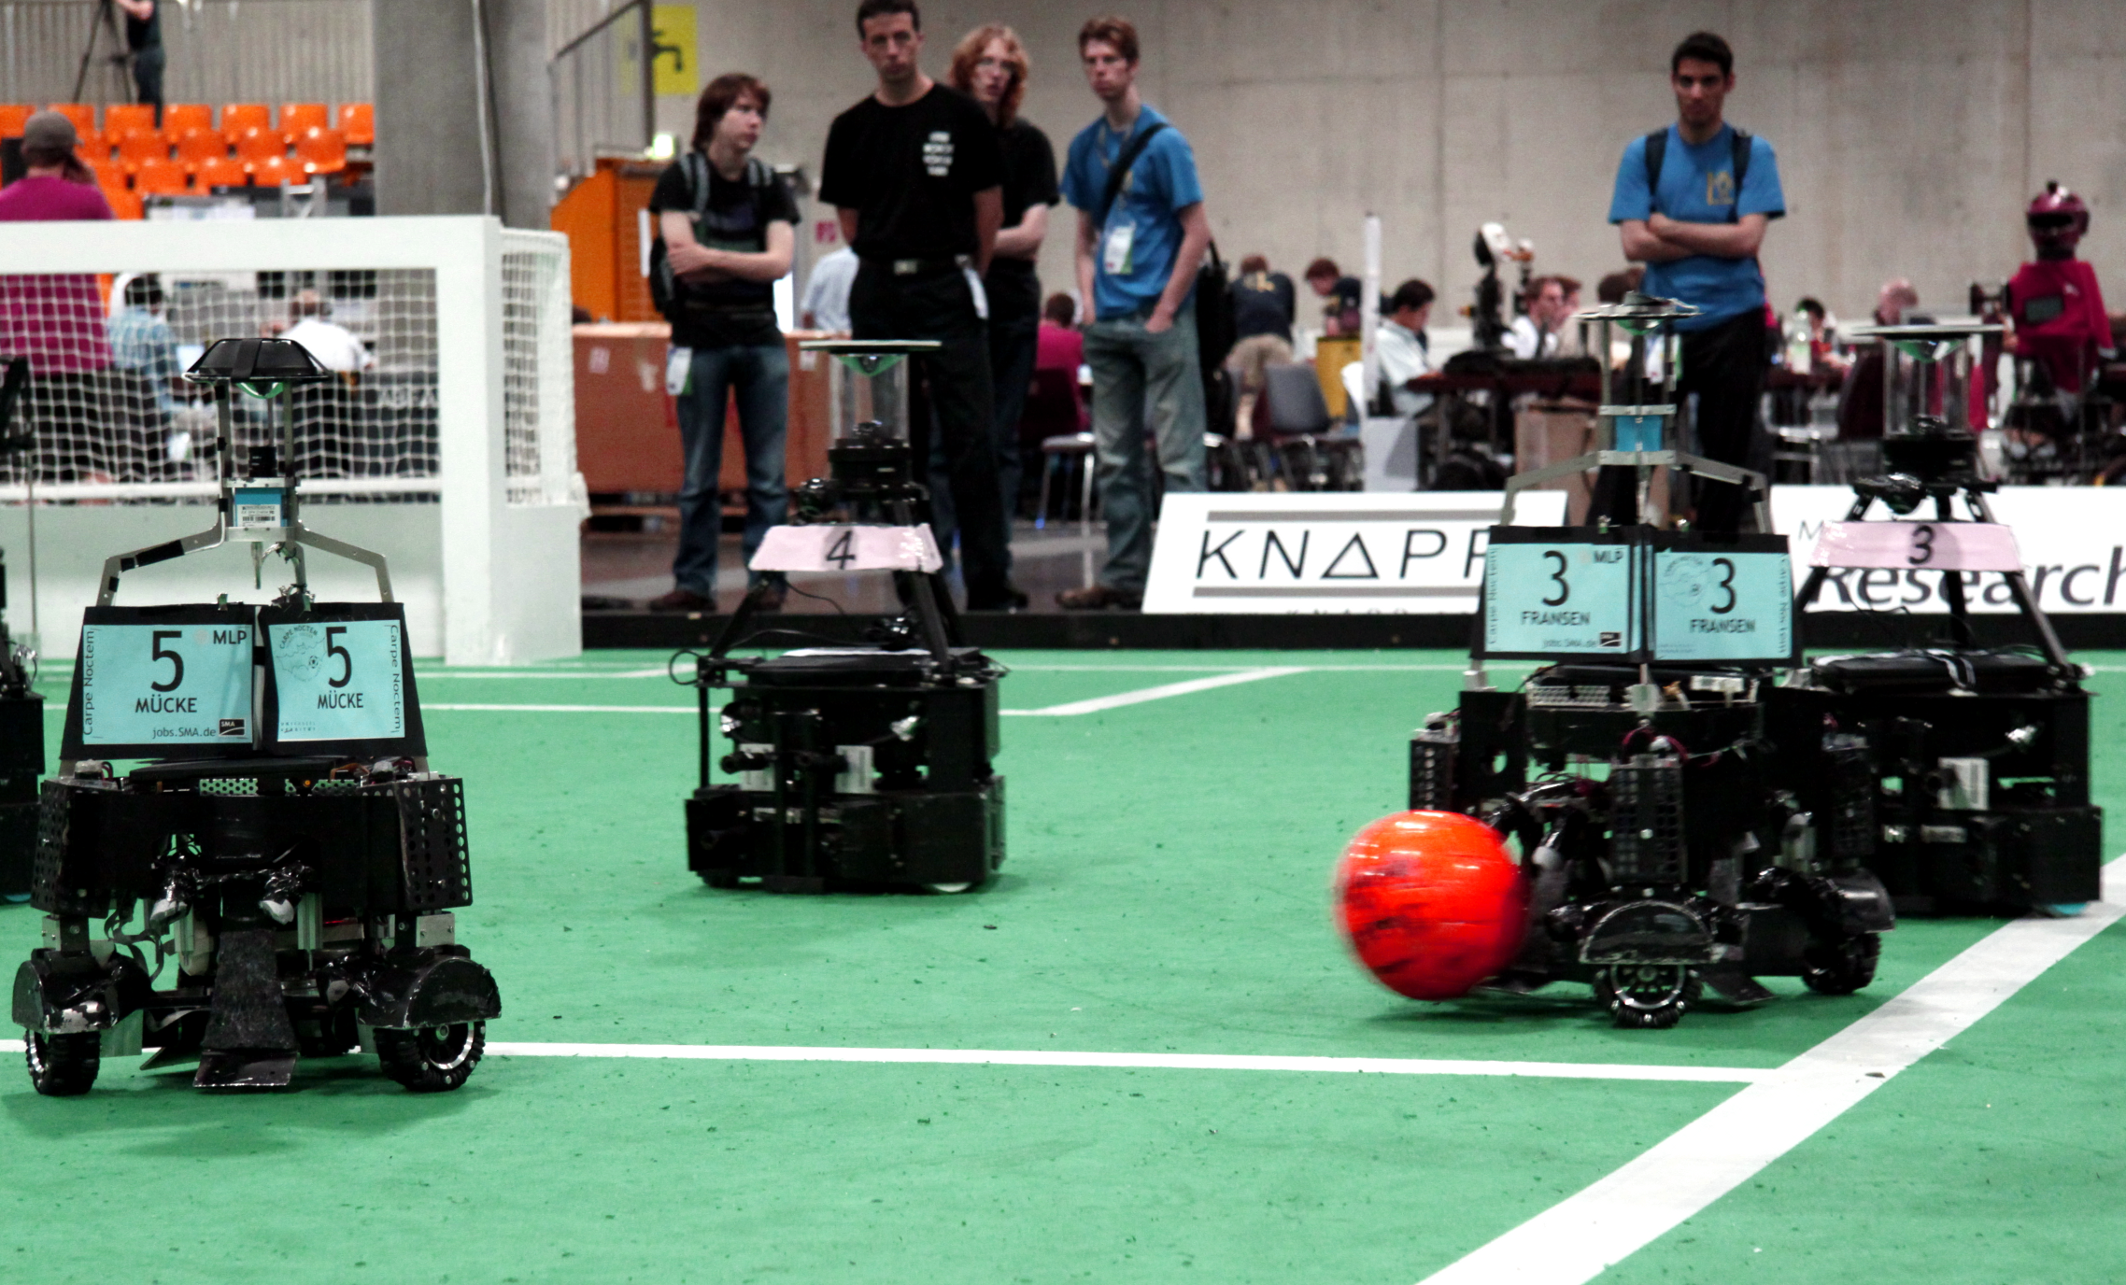
\includegraphics{./images/robots.png}
 % robots.png: 2126x1285 pixel, 300dpi, 18.00x10.88 cm, bb=0 0 510 308
 %\caption{Roboter Unfall}
 %\label{abb:test}
%\%end{wrapfigure}

 
Hier kommt ein bild von einem kaputten roboter hin, am besten mit beschreibung woran es lag und wie dieses mit meinem sys eventl. hätte verhindert 
werden können....da muss ich nochmal was zusammensuchen, ist eher optional...\\
\\

Durch die eingangs beschriebene Problemstellung ergeben sich mehrere zu lösende Aufgaben.
Es müssen Möglichkeiten untersucht werden verschiedene physikalische Größen, wie Spannungen oder Temperaturen mittels eines Mikrocontrollers zu messen.
Des weiteren soll der Mikrocontroller direkt eine entsprechende Reaktion durchführen, sollten die Messwerte bestimmte Schwellwerte unter- oder überschreiten. 
Zudem müssen die Daten in geeigneter Weise zum Robotersystem übertragen werden.\newline

Daraus wurden folgende Grundfunktionaltäten des Meßsystems abgeleitet:\newline
 

\begin{enumerate}
 \item Messen physikalischer Größen
 \item Kommunikation 
 \item Reaktionen durch das Meßsystem
\end{enumerate}

%\end{tabbing}



\chapter{Konzept}
\label{cha:Konzept}

Die Analyse der Problemstellung ergibt drei nötige Grundfunktionaltäten des zu entwickelden Systems. Diese sind voneinander unabhängig, 
daher werden die Konzepte zur Entwicklung der Funktionalitäten Messen, Kommunikation und Reaktion in den folgenden Unterpunkten getrennt diskutiert.\\
\begin{enumerate}
  \item Messen physikalischer Grössen\\
  Das Messen physikalischer Grössen erfolgt im Mikrocontrollerbereich entweder üder Spannungsmessungen, sollte der Sensor
  analoge Spannungswerte ausgeben oder über eine Bus-Kommunikation, beispielsweise I2C. Zur Spannungsmessung stellt der Mikrocontroller
  sogenannte ADC Eingänge zur Analog-/Digitalwandlung zur Verfügung.
  Diese Messwerte werden im Mikrocontroller mittels der im Datenblatt des Sensors festgelegten Formeln oder Tabellen ausgewertet.\\
  Spannungen in einem Robotersystem können in Bereichen von 1 bis über 300 V vorkommen, wobei die Standardspannungsbereiche 1, 5, 12 und 24 V betragen.
  Die Spannungsmessungen im Robotersystem erfordern daher die Möglichkeit verschiedene Spannungsbereiche messen zu können,
  um eine möglichst hohe Auflösung des Messbereichs zu gewährleisten. Da der Controller analoge Spannungswerte nur bis zu dessen Betriebsspannung (hier: 5V) verarbeiten kann, 
  müssen außerdem messtechnische Vorkehrungen getroffen werden, um den ADC Eingang des Controllers vor Spannungen über der Betriebsspannung zu schützen.
  Hier bieten sich verschiedene Methoden der Messtechnik an, um diese Funktionalitäten zu erreichen:
  \begin{itemize}
   \item  Verschiedene Spannungsteiler zur Einstellung der Messbereiche.
   \item  Externe Z-Dioden oder interne Schottky-Dioden des Controllers, zum Schutz des ADC Eingang des Controllers vor Überspannungen.
   \item  Verstärkerstufen, um auch sehr geringe Spannungen unter 1 V messen zu können.
  \end{itemize}

  
  \item Kommunikation\\
  
  fehlt noch
  
  \item Reaktionen durch Controller\\
Der Controller selbst kann eine Höchstlast von einigen mA schalten. Sollen größere Lasten geschaltet werden, muß der Controllerausgang
mit einer Schaltung versehen werden, die es ermöglicht diese großen Lasten zu schalten. Der Controller steuert in diesem Fall auschließlich einen elektronischen
Schalter(Transistor), dieser Schalter ist dafür zuständig die Last von der Spannungsversorgung zu trennen oder um einen weiteren noch leistungsfähigeren elektronischen Schalter(Relais) anzusteuern.
\end{enumerate}



\chapter{Umsetzung}
\label{cha:Umsetzung}
Wie wurden konzeptionelle Lösungen umgesetzt, Beschreibung in Arbeitsschritten...

Arbeitsschritte:

Darstellung der einzelnen Schritte


\chapter{Evaluierung}

\label{cha:Evaluierung}


Evaluierung der Funktionalitäten mittels verschiedener Versuchsaufbauten und anschliessender Dokumentation
der Messreihen...

\begin{center}
Messreihe 5 V Messungen:
\begin{tabular}{lllllll}
Spannungswert & Messung  0 & Messung 2 & Messung 3 & Messung 4 & Messung 5 & Messung 6\\
0 V & 0 & 0 & 0 & 0 & 0 & 0\\
1,3 V & 0 & 0 & 0 & 0 & 0 & 0\\
2,5 V & 0 & 0 & 0 & 0 & 0 & 0\\
3,5 V & 0 & 0 & 0 & 0 & 0 & 0\\
4,9 V & 0 & 0 & 0 & 0 & 0 & 0
\end{tabular}
\end{center}



\chapter{Zusammenfassung}
\label{cha:Zusammenfassung}
Zusammenfassung .... es funktioniert :-D

\chapter{Abbildungsverzeichnis}
\label{cha:Abbildungsverzeichnis}

\chapter{Literaturverzeichnis}

\bibliographystyle{plainnat}
%\bibliography{bibtex_database}

\end{document}
